
\section{Introduction}
\label{sec:Introduction}
%%%%%%%%%%%%%%%%%%%%% Vision %%%%%%%%%%%%%%%%%%%%%%%%%
The goal of this work is to describe several fabrication methods for various kinds of soft robots.
Each fabrication method produces one or several unit-modules that can be actuated based on the soft fluidic elastomer model.
Each fabrication process can be used to create actuatable soft modules; these modules can be composed in series or in parallel to create a range of different soft robot morphologies.
%The goal of this work is to provide and compare multiple actuator morphologies and multiple fabrication processes for realizing soft autonomous fluidic elastomer robots.
%
We experimentally validate these morphologies in the context of extremely soft and highly compliant locomotory robots and manipulators shown in Figure~\ref{fig:intro_new}.

\begin{figure}[!t]
  \centering
  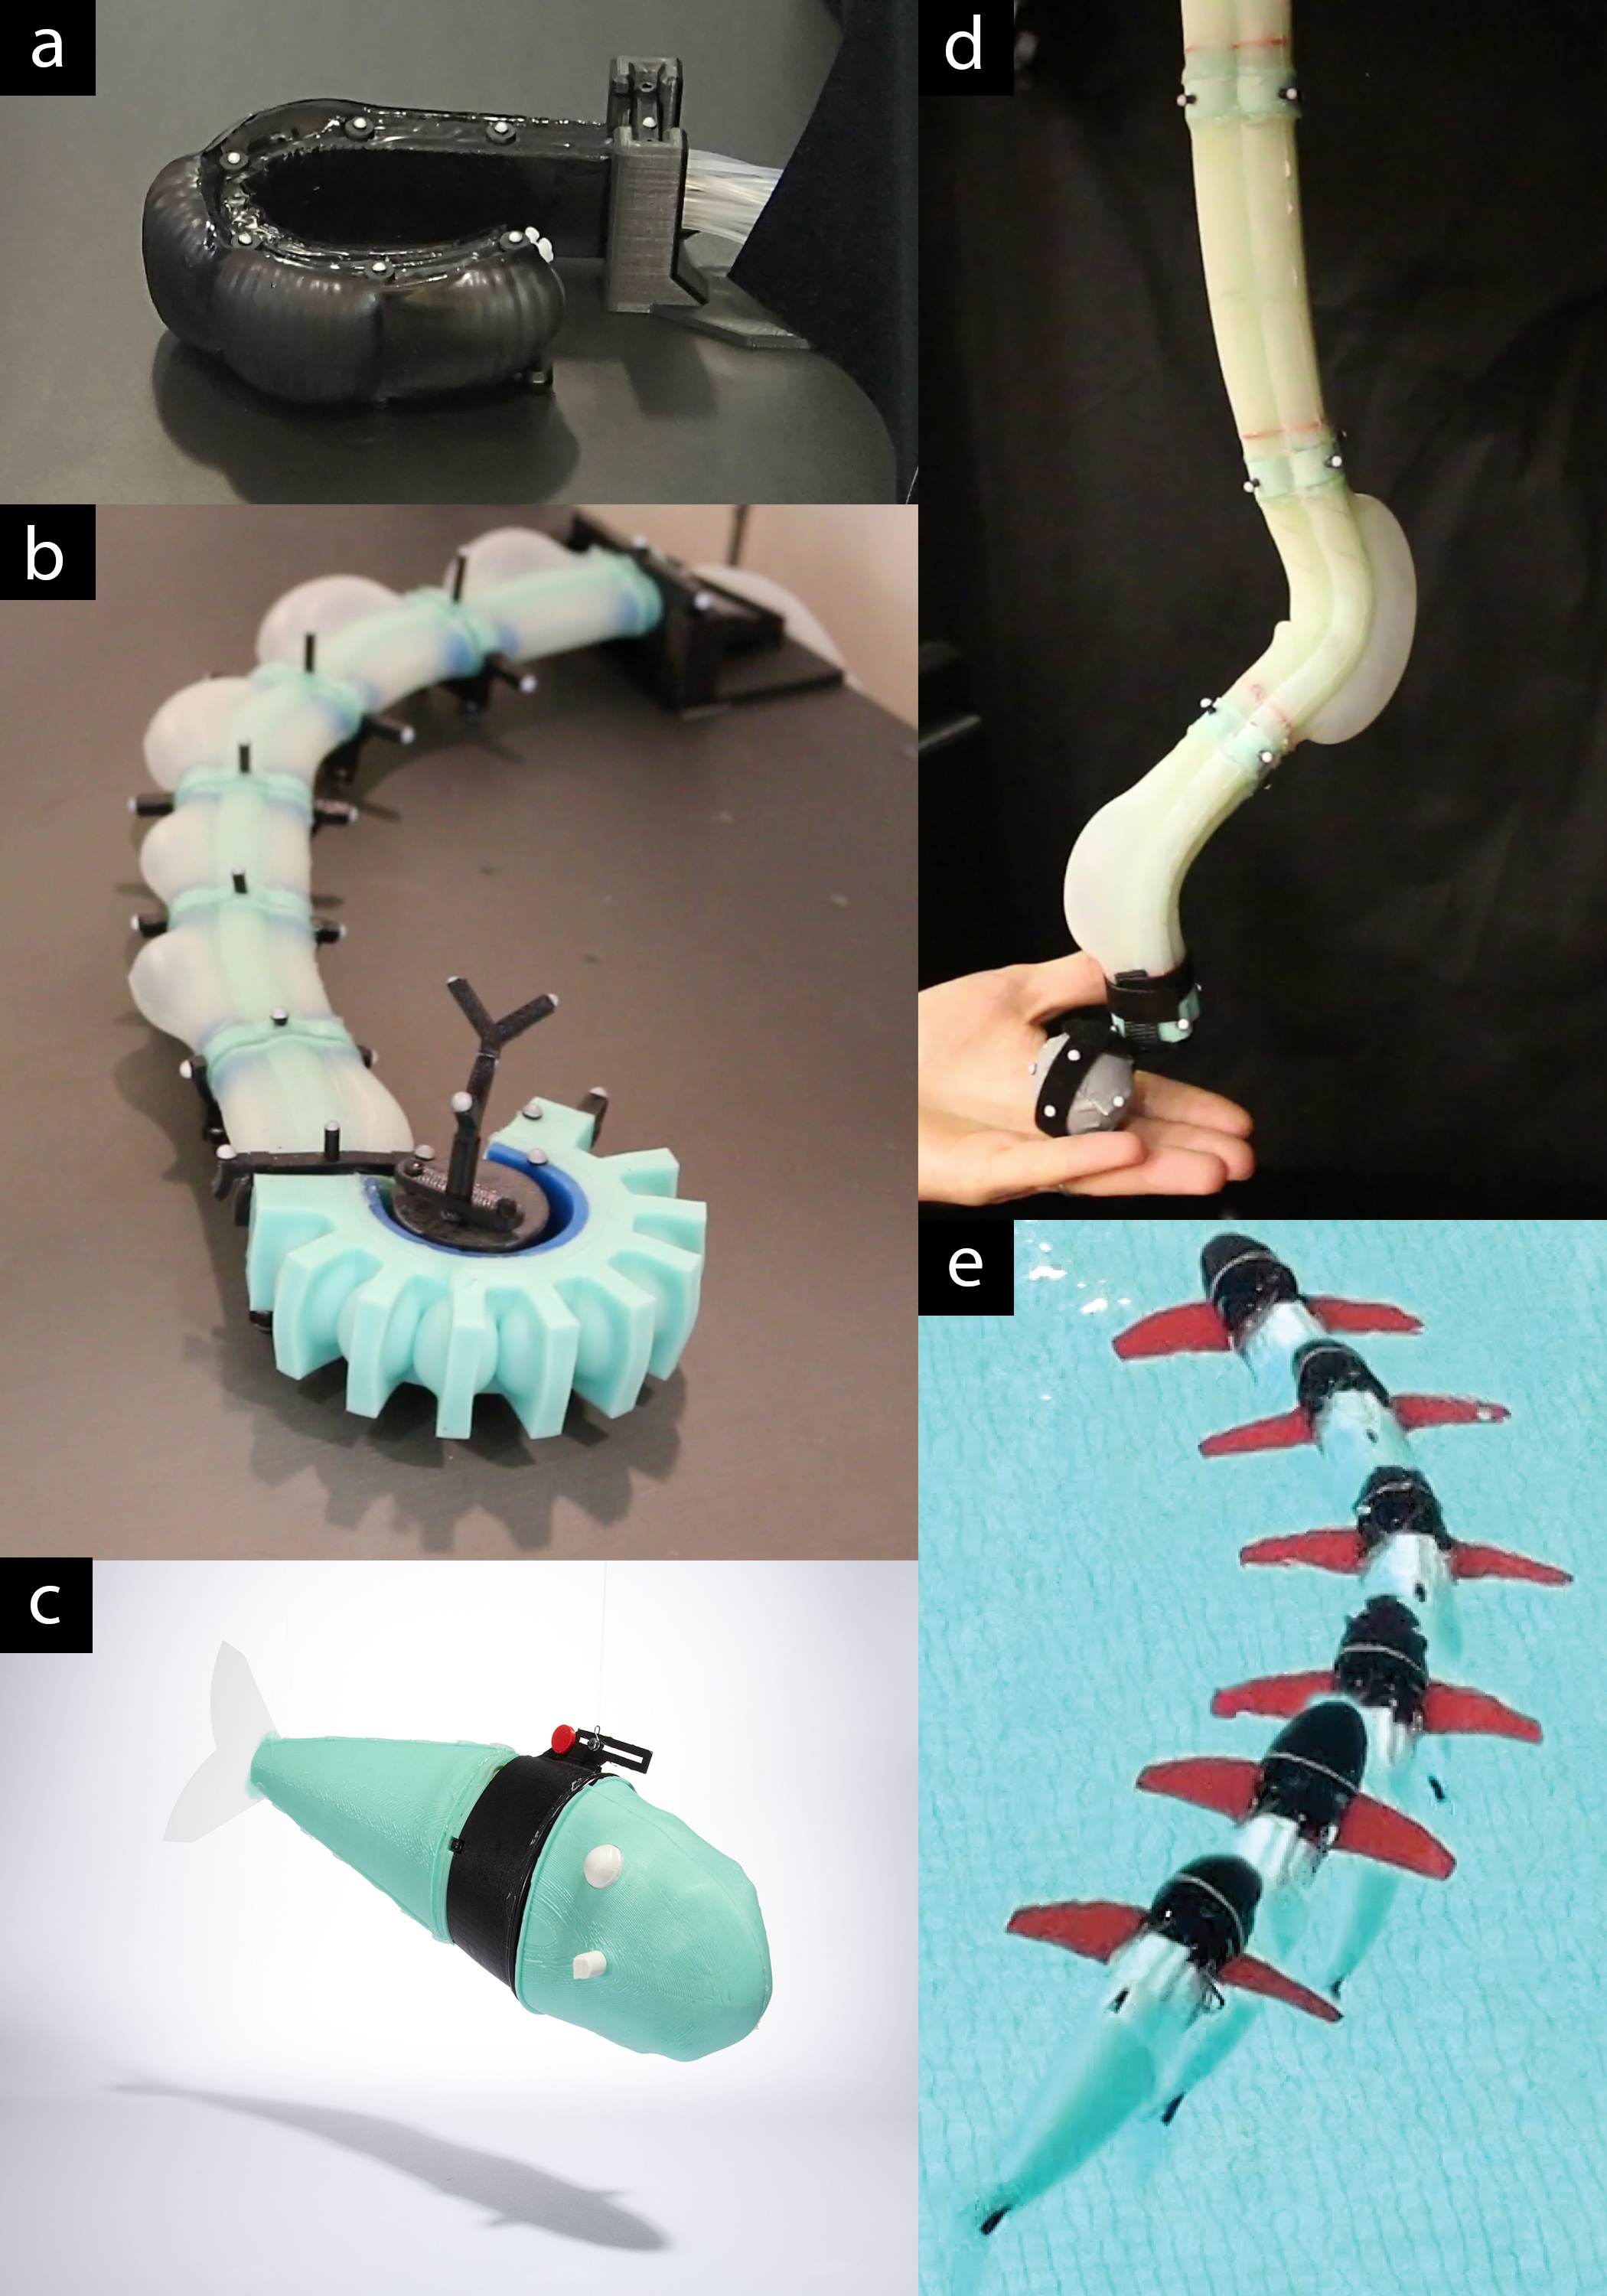
\includegraphics[width=3in]{figures/introduction/intronew_v2.jpg}
  \caption{Extremely soft and highly compliant fluidic elastomer robots. (\textbf{a}) Ribbed planar manipulator \citep{marchese2014design}, (\textbf{b}) Cylindrical manipulator with gripper \citep{katzschmann2015autonomous}, (\textbf{c}) Self-contained pneumatic fish \citep{marchese2014autonomous}, (\textbf{d}) Spatial cylindrical manipulator \citep{marchese2015design}, and (\textbf{e}) Self-contained hydraulic fish \citep{katzschmann2014hydraulic}. }\label{fig:intro_new}
\end{figure}
%REMOVED: (\textbf{b}) Cylindrical planar manipulator \citep{marchese2014whole}

Soft robots exhibit continuum body motion, large scale deformation, and relatively high compliance compared to traditional rigid-bodied robots \citep{trivedi2008soft}.
%
Such characteristics give this class of robots advantages like the ability to mitigate uncertainty with passive compliance \citep{mcmahan2006field}, perform highly dexterous tasks \citep{deimel2014novel}, and exhibit resiliency \citep{tolley2014resilient}.
%
This work provides a recipe for designing and fabricating soft fluidic elastomer actuators and robotic systems. %NOTE: This sent does not really fit well at this point, might want to move it upwards into the first paragraph...

%%%%%%%%%%%%%%%%%%%%% Challenges %%%%%%%%%%%%%%%%%%%%%%%%%
%\subsection{Challenges}
Recent reviews \citep{trivedi2008soft, trimmer2014journal, lipson2014challenges, majidi2014soft} articulate the challenges associated with creating robots from soft, nonlinear materials.
%
Current engineering tools are well-suited for rigid-bodied robots and when soft, nonlinear elastic materials are introduced, many of the underlying assumptions of these tools are not valid anymore.
%
To create fluidic elastomer robots, we must overcome many technical challenges:
(i) We need methods for composing soft-unit modules to create complex morphologies suitable for robot bodies capable of autonomous locomotion and manipulation.
That is, we need to identify appropriate modules and ways of assembling these into multi-body robots.
(ii) Consistently reproducing certain properties of soft robots, for example their elasticity or internal channel geometry, is difficult using conventional fabrication techniques.
Accordingly, we must develop fabrication techniques that balance the competing goals of scalability and repeatability with the need for complicated features and shape profiles.

%%%%%%%%%%%%%%%%%%%%% Contributions %%%%%%%%%%%%%%%%%%%%%%%%%
%The primary contribution of this work is a novel power and computational control and planning system for 2D fluidic elastomer manipulation that enable grasp-and-place and planned continuous motion in environments with obstacles.
%This work is first to show that planar manipulation with soft fluidic elastomer robots is possible and first to provide an approach for closed-loop control and planning of such manipulators.
This work makes the following contributions:
\begin{enumerate}
 \item Classification of three viable fluidic elastomer actuator (FEA) morphologies. That is, an FEA with a (i) ribbed channel structure and embedded transmission lines, (ii) cylindrical channel structure and hollow interior, (iii) seamless pleated channel structure;
 \item Three fabrication processes to reliably manufacture these FEAs. These are (i) a lamination-based casting process with heterogeneous embedded components, (ii) a retractable-pin-based casting process, (iii) a lost-wax-based casting process;
 \item A survey of recent robots built using these design and fabrication approaches.
\end{enumerate}
This work significantly extends four previous conference publications: \citep{marchese2014design}, \cite{katzschmann2014hydraulic}, \citep{marchese2014whole}, and \citep{katzschmann2015autonomous}.

%%%%%%%%%%%%%%%%%%%%% Approach %%%%%%%%%%%%%%%%%%%%%%%%%
%In this work, we demonstrate that autonomous manipulation with soft fluidic elastomer robots is possible.
This paper is organized as follows.
First, we review relevant soft actuation technology, design tools, and fabrication processes in Section~\ref{sec:Related Work}.
%
Next, we present the design and characterization of three fluidic elastomer actuator morphologies in Section~\ref{sec:Actuators}.
%
These actuator morphologies are differentiated by their internal channel structure, namely: ribbed, cylindrical, and pleated.
%
Next, we provide three alternative fabrication approaches for reliably fabricating soft actuators and multi-segment robots in Section~\ref{sec:Fabrication}.
%
These processes are lamination-based embedded casting, retractable-pin-based casting, and lost-wax-based casting.
%
Then, we briefly discuss alternative approaches to powering these robots in Section~\ref{sec:Power}.
%
And lastly, we demonstrate how the various actuator morphologies and fabrication processes have been used to realize a variety of soft autonomous systems: locomotory fish-like robots in Section~\ref{sec:Locomotion} and robotic manipulation systems in Section~\ref{sec:Manipulators}. 